\section{Metodología}
Es difícil encontrar una definición estándar para una metodología de desarrollo de software, Centers for medicare \& medicaid services o CMS (2017), definen una metodología de desarrollo de software como “un marco de trabajo que es usado para estructurar, planificar y controlar el proceso de desarrollo de un sistema de información”\cite{metodologia}.
\\
\textbf{Modelo Incremental}\\
El modelo incremental combina elementos de los flujos de proceso lineal y paralelo, el modelo incremental aplica secuencias lineales en forma escalonada a medida que avanza el calendario de actividades. Cada secuencia lineal produce “incrementos” de software susceptibles de entregarse.\\
Cuando se utiliza un modelo incremental, es frecuente que el primer incremento sea el producto fundamental. Es decir, se abordan los requerimientos básicos, pero no se proporcionan muchas características suplementarias. El modelo de proceso incremental se centra en que en cada incremento se entrega un producto que ya opera. Los primeros incrementos son versiones desnudas del producto final, pero proporcionan capacidad que sirve al usuario y también le dan una plataforma de evaluación.\\
El desarrollo incremental es útil en particular cuando no se dispone de personal para la implementación completa del proyecto en el plazo establecido por el negocio. Los primeros incrementos se desarrollan con pocos trabajadores. Si el producto básico es bien recibido, entonces
se agrega más personal (si se requiere) para que labore en el siguiente incremento. Además, los incrementos se planean para administrar riesgos técnicos.\cite{Pressman}.
\\
En la imagen \ref{fig:ModeloIncremental} se muestra el modelo incremental.
\begin{figure}[H]
	\centering
	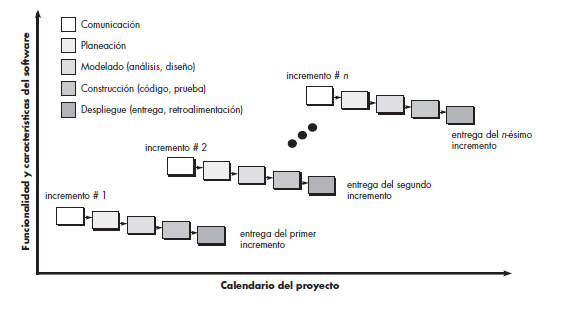
\includegraphics[width=1\textwidth]{Capitulo3/img/ModeloIncremental}
	\caption{Modelo Incremental}
	\label{fig:ModeloIncremental}
\end{figure}

Este tipo de modelo se utilizará debido a que los incrementos nos permiten desarrollar el sistema desde su parte mas fundamental hasta tener el sistema completo y funcionando, obteniendo un entregable en cada uno de los incrementos.
\\
Los incrementos que se realizarán serán los siguientes:
\\
\begin{enumerate}
	\item Se realizará el módulo del sensor el cual consiste en el análisis del sensor de flujo, del microcontrolador a utilizar y la forma de comunicación con la aplicación móvil para el envío del dato de la medición obtenida.
	\item Se hará el diseño y programación para realizar la comunicación entre el sensor y la aplicación y se realizarán las pruebas unitarias pertinentes para asegurar que la medición y comunicación sean correctos.
	\item Se realizará módulo de la aplicación móvil el cual consiste en el análisis y diseño de la aplicación móvil para la obtención de datos, se realizará la programación de la interfaz de la aplicación móvil con la cual el usuario podrá visualizar los datos y se realizaran las pruebas pertinentes.
	\item Se continuará con el análisis, diseño y programación del submódulo de usuarios, en el cual se tendrá una aplicación móvil en la cual el usuario pueda interactuar de una forma fácil y eficiente con el sistema.
	\item Se realizará el análisis, diseño y programación del submódulo para la geolocalización de los establecimientos.
	\item Se realizara el análisis y diseño para el envío y recepción de datos entre la aplicación móvil y el servidor web y se realizarán las pruebas de integración de todo el módulo de la aplicación móvil.
	\item Se realizará el módulo servidor web el cual consiste en el análisis, diseños y programación de la recepción de los datos obtenidos, asimismo se realizarán las pruebas unitarias del incremento en cuestión.
	\item Se continuará con el módulo servidor web con el análisis, diseño y programación para la clasificación de los establecimientos según los resultados obtenidos y se realizarán tanto pruebas unitarias del módulo servidor web..
	\item En este incremento se harán las pruebas de integración del sistema.	
\end{enumerate}
